\documentclass[a4paper,12pt]{article}
\usepackage[T1,T2A]{fontenc}
\usepackage[utf8]{inputenc}
\usepackage[english,ukrainian]{babel}


\usepackage{ upgreek }
\usepackage{amsmath}

\usepackage{graphicx}
\graphicspath{{./pictures/}}


\usepackage[unicode=true,colorlinks=true,urlcolor=blue,citecolor=green,linkcolor=blue]{hyperref}
\usepackage[ukrainian,nameinlink]{cleveref}
\usepackage{geometry} % Меняем поля страницы
\geometry{left=2cm}% левое поле
\geometry{right=1.5cm}% правое поле
\geometry{top=1cm}% верхнее поле
\geometry{bottom=2cm}% нижнее поле



\begin{document}
	
	\begin{titlepage}
		\vspace*{6cm}
		\begin{center}
			
			\large
			\textbf{Звіт}\\
			\textbf{до лабораторної роботи №3:}\\
			\textbf{<<Відстань Махаланобіса>>}
			
		\end{center}
		
		\vspace{8cm}
		\begin{flushright}
			студента 1-го курсу магістратури\\
			факультету комп'ютерних наук та кібернетики\\
			Кравця Олексія
		\end{flushright}
		
	\end{titlepage}

\newpage
\tableofcontents
\newpage
%document here
\section{Постановка задачі}

Маємо 3 множини точок, кожна з яких представляє один з типів результату (Тип 1, Тип 2, Тип 3).

Необхідно згенерувати набір точок і класифікувати кожну точку. Приймати рішення про приналежність точки до одного з трьох типів будемо на основі відстані Махаланобіса.

\subsection{Означення}

Відстань Махалонобіса - міра відстані між векторами випадкових величин, що узагальнює поняття евклідової відстані \cite{Wiki}.

Формально відстань Махалонобіса від вектора $x= (x_1, \ldots, x_N)^T$ до множини із середнім значенням $\mu = (\mu_1, \ldots, \mu_N)^T$ та матрицею коваріації $S$. Визначається наступним чином

\begin{equation}
	D_M (x, \mu) = \sqrt{(x-\mu)^T S^{-1} (x-\mu)}
\end{equation}

\section{Виконання роботи}

Зу умовою, точки Типу 1 і Типу 3 мають рівномірний розподіл, а точки Типу 2 -- нормальний. Отже оберемо такі типи
\begin{itemize}
	\item Тип 1. Рівномірний розподіл. Точки лежать всередині $(x,y) \in [3,4) \times [4,5)$;
	\item Тип 2. Нормальний розподіл. Його точки мають такі властивості  $\mu_x = 1, \sigma_x = 0.1$ по $x$ та $\mu_y = 1, \sigma_y = 0.7$ по $y$;
	\item Тип 3. Рівномірний розподіл. Точки лежать всередині $(x,y) \in [5,6) \times [0,1)$.
\end{itemize}

Згенеруємо по $N=20$ точок кожного типу.

\begin{figure}[h!]
	\center{ 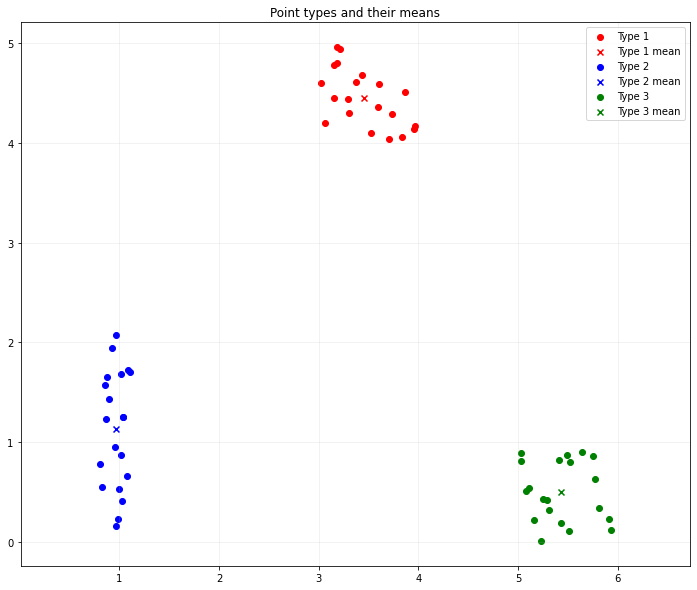
\includegraphics[scale=0.4]{fig_1.png}}
	\caption{Точки типів}
\end{figure}

Тепер згенеруємо $100$ тестових точок.

\begin{figure}[h!]
	\center{ 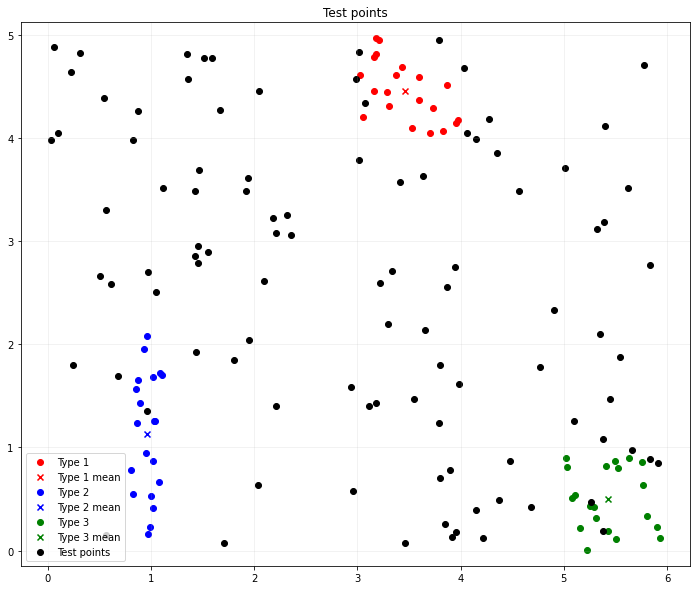
\includegraphics[scale=0.7]{fig_2.png}}
	\caption{Тестові точки}
\end{figure}

\newpage
Класифікуємо точки.

\begin{figure}
	\center{ 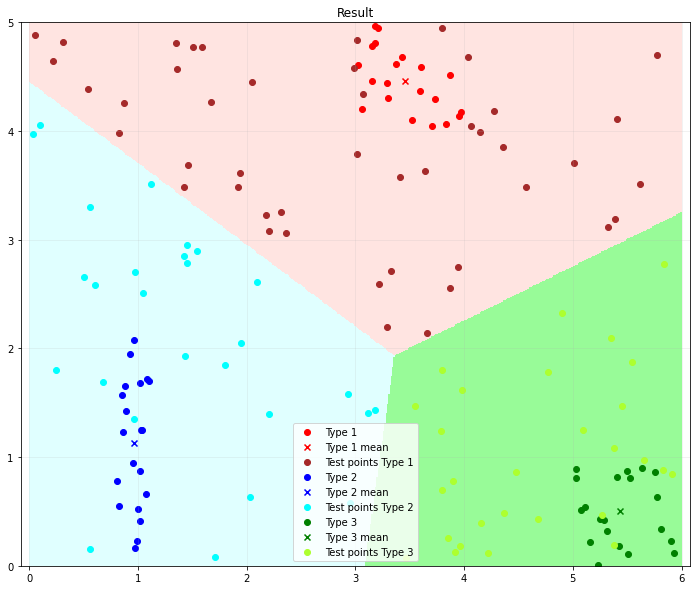
\includegraphics[scale=0.7]{fig_4.png}}
	\caption{Тестові точки}
\end{figure}


\newpage
\addcontentsline{toc}{section}{Література}
\begin{thebibliography}{}
	\bibitem{Wiki} \href{https://en.wikipedia.org/wiki/Mahalanobis_distance}{https://en.wikipedia.org/wiki/Mahalanobis\_distance}
\end{thebibliography}

\end{document}
